\section{Teoría de Acoplamiento}\cite{yariv2006photonics}
\label{coupling_theory}

En la figura \ref{fig:rr_model} se muestra el esquema del caso genérico de un anillo resonador con 2 regiones de acoplamiento representadas por las líneas punteadas. 
Por simplicidad, el modelo asume que no hay pérdidas por 
acoplamiento (\ref{eq:energy_conserv}) y se ignoran los efectos de reflexión 
dentro de la guía (sólo se asumen ondas en el sentido de la propagación). 

Cada región tiene asociados 
coeficientes de acoplamiento $(\kappa_1,\kappa_1^{'}\kappa_2\kappa_2^{'})$ y
coeficientes de transmisión $(t_1, t_1^{'}, t_2, t_2^{'})$ que posteriormente
serán relacionados entre si (sección \ref{ss:params_relation}).


\begin{figure}[h!]
\caption{Modelo de un Anillo Resonador}
\centering
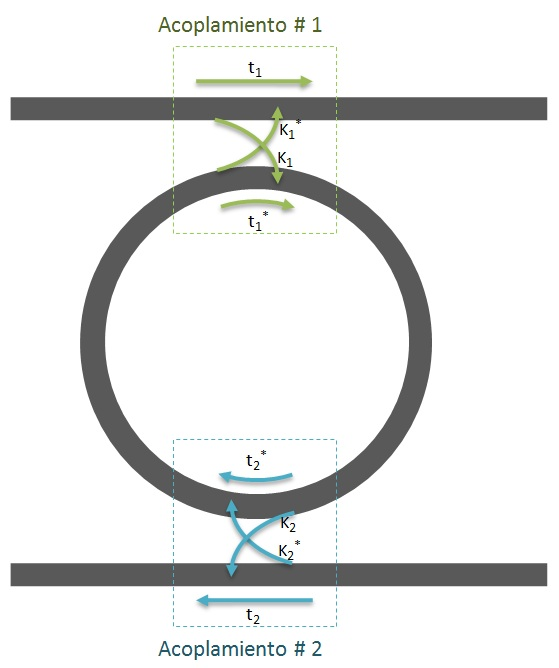
\includegraphics[width=0.5\textwidth,natwidth=559,natheight=668]{figs/rr_model.jpg}
\label{fig:rr_model}
\end{figure} 


La potencia de la onda que se ve en el $puerto_t$ está dada por la porción de la onda incidente
que atravieza la guía más las $N\to\infty$ contribuciones que se dan por la otra parte de la
onda que se acopló en el anillo (ec. \ref{eq:coupling_gral}). 
Cada una de las contribuciones depende del número de viajes completos que realice la onda
acoplada antes de volver a salir a la guía superior.


\begin{equation}
E_t = E_i t_1 + Contrib_{N=1L} + Contrib_{N=2L} + ... + Contrib_{N=\infty L}
\label{eq:coupling_gral}
\end{equation} 

\begin{itemize}
\item Contribución después de una vuelta: $Contrib_{N=1L}$
\end{itemize} 


\begin{figure}[h!]
\caption{Contribución Onda 1 Vuelta}
\centering
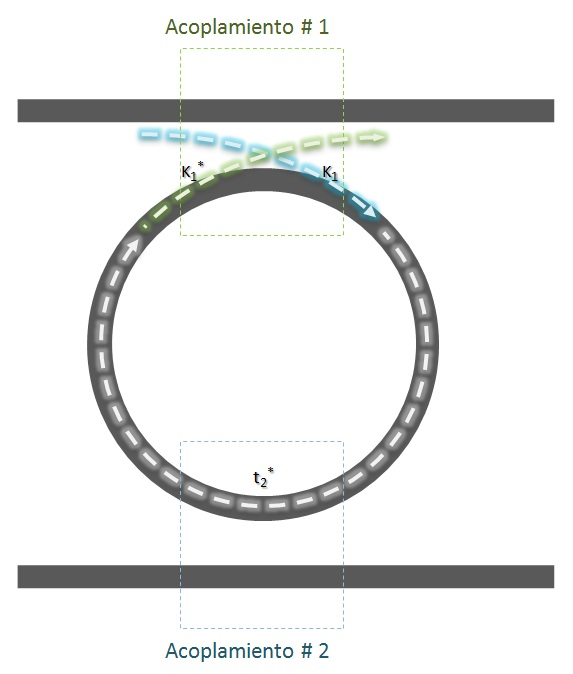
\includegraphics[width=0.5\textwidth,natwidth=573,natheight=674]{figs/rr_n1.jpg}
\label{fig:rr_n1}
\end{figure} 

El fasor escalar $\alpha e^{-j \beta L}$ contiene la información sobre la amplitud de
la atenuación (debido a efectos de dispersión y a la curvatura de la onda) 
y la fase de la onda que ha recorrido una distancia L, 
donde L representa el perímetro ($2 \pi r$) del anillo con radio $r$. 
Por lo tanto, al dar una vuelta ($1L$), la propagación de la onda queda expresada como 
$\alpha e^{-j \beta L}$.

En su recorrido completo, la onda que da una vuelta completa (Figura \ref{fig:rr_n1}) 
pasa por 3 regiones de interés. 
En la primera región (acoplamiento 1) una porción (dada por el factor de acoplamiento 
$\kappa_1$) entra desde la guía recta hacia el anillo.
En la segunda región (acoplamiento 2), una porción (dada por el factor de transmisión 
$t_2^{'}$) continúa su viaje al interior del anillo.
Finalmente, en la tercera región (acoplamiento 1) sólo una parte de la onda (dada por la 
conjugada del factor de acoplamiento ó $\kappa_1^{'}$) vuelve a la guía original para 
salir por el $puerto_t$. 


Teniendo en cuenta cada una de estas atenuaciones más el fasor que expresa la propagación
de la onda, se llega a (\ref{eq:coupling_round_1}).

\begin{equation}
Contrib_{N=1L} = E_i \alpha e^{-j \beta L} \kappa_1 t_2^{'} \kappa_1^{'}
\label{eq:coupling_round_1}
\end{equation} 

\begin{itemize}
\item Contribución después de dos vueltas: $Contrib_{N=2L}$
\end{itemize} 

Se analizará la parte de la onda que no se reintegró a la guía recta tras la primera vuelta
y que da otra vuelta antes de volver a la guía recta para salir por el $puerto_t$
(Figura \ref{fig:rr_n2}).
La propagación de la onda tras 2 vueltas completas ($2L$), está dada por 
$\alpha^2 e^{-j \beta 2L}$.
La onda atravieza 2 nuevas regiones (aparte de las 3 regiones mencionadas en la sección anterior)
por cada nueva vuelta que deba dar. 

La primera es la región de acoplamiento 1 (en una proporción dada por $t_1^{'}$) 
para seguir su trayectoria dentro del anillo.
La segunda es la región de acoplamiento 2, la cual debe atravezar (según el factor de transmisión $t_2^{'}$).

Estas nuevas atenuaciones se ven reflejadas en (\ref{eq:coupling_round_2}). 
El término $\alpha^2 e^{-2j \beta L}$ se expresó como
 $\alpha e^{-j \beta L} \alpha e^{-j \beta L}$ para facilitar
su generalización posterior.

\begin{figure}[h!]
\caption{Contribución Onda 2 Vueltas}
\centering
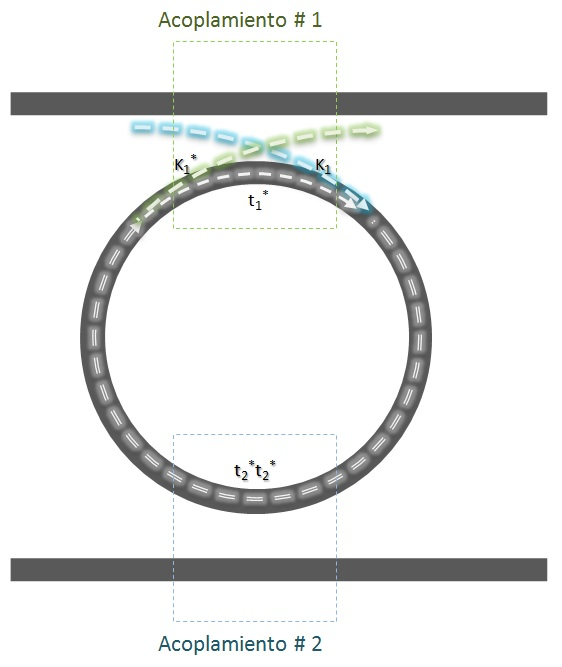
\includegraphics[width=0.5\textwidth,natwidth=562,natheight=667]{figs/rr_n2.jpg}
\label{fig:rr_n2}
\end{figure} 

\begin{equation}
Contrib_{N=2L} = E_i \alpha e^{-j \beta L} \kappa_1 t_2^{'} \kappa_1^{'} (\alpha e^{-j \beta L} t_1^{'} t_2^{'})
\label{eq:coupling_round_2}
\end{equation} 

\begin{itemize}
\item Contribución después de N vueltas: $Contrib_N$
\end{itemize} 

Por cada vuelta adicional antes de acoplarse, se deben tener en cuenta los 
coeficientes de transmisión en estas 2 regiones más el desfase y la atenuación de la 
onda en cada vuelta (\ref{eq:coupling_round_n}).

\begin{equation}
Contrib_N = E_i \alpha e^{-j \beta L} \kappa_1 t_2^{'} \kappa_1^{'} (\alpha e^{-j \beta L} t_1^{'} t_2^{'})^{N-1}
\label{eq:coupling_round_n}
\end{equation} 

Sustituyendo la expresión para cada una de las contribuciones en 
(\ref{eq:coupling_gral}) y reorganizando, se llega a (\ref{eq:coupling_sum}).


\begin{equation}
E_t = E_i\{
t_1+
\kappa_1\kappa_1^{'} t_2^{'} \alpha e^{-j \beta L} [
1 +
(t_1^{'} t_2^{'} \alpha e^{-j \beta L})^1 +
(t_1^{'} t_2^{'} \alpha e^{-j \beta L})^2 +
...]\}
\label{eq:coupling_sum}
\end{equation}

Al ser una serie geométrica infinita, su solución está dada por (\ref{eq:geom_series}).

\begin{equation}
\sum\limits_{k = 0}^\infty {ar^{k} = \frac{a}{{1 - r}}}, \text{ si } |r| < 1
\label{eq:geom_series}
\end{equation} 

Sea 
$a = \kappa_1 \kappa_1^{'} t_2^{'} \alpha e^{-j \beta L} $ y  
$r = t_1^{'} t_2^{'} \alpha e^{-j \beta L}$.
Por lo tanto:

\begin{align}
E_t &= E_i\{t_1 + 
\frac{ \kappa_1 \kappa_1^{'} t_2^{'} \alpha e^{-j \beta L}}
{1 - t_1^{'} t_2^{'} \alpha e^{-j \beta L}} \} \\
\frac{E_t}{E_i} &= 
    \frac{t_1 + (\kappa_1 \kappa_1^{'} - t_1 t_1^{'})t_2^{'} \alpha e^{-j \beta L}}
    {1 - t_1^{'} t_2^{'} \alpha e^{-j \beta L}}
\label{eq:t_through}
\end{align} 

El cálculo de la potencia transmitida en el $puerto_d$ sigue una
lógica similar (\ref{eq:t_drop}).

\begin{equation}
\frac{E_d}{E_i} = \frac{ \kappa_1 \kappa_2^{'} \alpha e^{ -j \beta \frac{L}{2}} }
	   { 1 - t_1^{'} t_2^{'} \alpha e^{-j \beta L} }
\label{eq:t_drop}
\end{equation} 

\subsection{Relación entre Coeficientes de Acoplamiento}
\label{ss:params_relation}

Como se explica en \cite{yariv2006photonics}, los 4 coeficientes de transmisión más
los 4 coeficientes de acoplamiento no son independientes entre si, sino que están
relacionados por los principios fundamentales de reciprocidad, conservación de la energía
y T-simetría. Adicionalmente, como se mencionó en el apartado anterior, el sistema
asume que no hay pérdidas por inserción (\ref{eq:energy_conserv}).

\begin{align}
|t_1|^2 + |\kappa_1|^2 = |t_1^{'}|^2 &+ |\kappa_1^{'}|^2 = 1  \label{eq:energy_conserv} \\
t_1 t_1^{'} - \kappa_1 \kappa_1^{'} &= -1 \label{eq:unitary_matrix} \\
t_1 = |t_1|& e^{j \phi_{t_1}}
\end{align} 

\begin{equation}
    \left[ \begin{array}{c} E_s \\ E_{sk} \end{array} \right] 
    = 
    \begin{bmatrix} t_1 & k_1^* \\ k_1 & -t_1^* \end{bmatrix} 
    \times 
    \left[ \begin{array}{c} E_i \\ E_{ik} \end{array} \right]
\label{eq:eqname}
\end{equation} 

Reemplazando (\ref{eq:unitary_matrix}) en (\ref{eq:t_through}) se encuentra la
expresión para la amplitud normalizada en el $puerto_t$ (ec. \ref{eq:t_through_simp}).

\begin{align}
\frac{E_t}{E_i} &= 
    \frac{t_1 - t_2^* \alpha e^{-j \beta L}}
    {1 - t_1^* t_2^* \alpha e^{-j \beta L}} \label{eq:t_through_simp}
\end{align} 

La función de transmisión en $puerto_t$ está dada por (\ref{eq:T_t}) \cite{paloczi2005polymer}.

\begin{align}
 T_t &= \abs*{\frac{E_t}{E_i}}^2 = 
    \frac{\alpha^2 |t_2^*|^2 + |t_1^*|^2 - 2\alpha |t_1^*||t_2^*| 
	\cos(\theta + \phi_{t_1} + \phi_{t_2}) }
    {1 + \alpha^2|t_1^*|^2 |t_2^*|^2 - 2\alpha |t_1^*||t_2^*|
	\cos(\theta + \phi_{t_1} + \phi_{t_2}) }
\\ 
\label{eq:T_t}
\end{align} 
